\section{Dati e analisi}
Con le impostazioni che ho ricavato nella sezione precedente ho quindi proceduto con la simulazione del comportamento delle onde in presenza di vari potenziali.
\subsection{Il salto di potenziale}
Il primo potenziale che analizzo \`e il salto di potenziale, posiziono un gradino a met\`a del dominio e variandone l'altezza ne calcolo il coefficiente di trasmissivit\`a.

\begin{equation}
  \lr\{.{\begin{array}{lr}
      V_0& x>a\\
      0&\text{altrove}
  \end{array}}
\end{equation}

Prima di tutto far\`o una piccola parentesi teorica sul risultato che mi aspetto. Prendiamo un dominio infinito con in 0 il salto di potenziale, l'equazione, indipendente dal tempo, avr\`a la forma:
\begin{equation}
  E\psi = \lrt{-\frac{\hbar^2}{2m}\pde{^2}{x^2}+V_0H(x)}\psi
\end{equation}
Divido lo spazio in due porzioni ($x<0$ e $x>0$) in cui:
\begin{equation}\label{eq:Ks}
  \begin{array}{lr}
    k_1 = \sqrt\frac{2m E}{\hbar^2}&x<0\\
    k_2 = \sqrt\frac{2m \lrt{E-V_0}}{\hbar^2}&x>0
  \end{array}
\end{equation}
Dato che il potenziale ha una discontinuit\`a finita in $0$, funzione e derivata devono essere continue. Se per esempio avessimo delle onde piane in ciascuna porzione dello spazio ne avrei una che si muove verso destra ($\psi_\to$) e una verso sinistra ($\psi_\from$) e quindi in 0 avrei, chiamando i coefficenti delle onde piane $A$ per il lato sinistro e $B$ quello destro:
\begin{equation}
  \lr\{.{\begin{array}{lr}
      A_\to e^{ik_1x} + A_\from e^{-ik_1x}	&	x<0\\
      B_\to e^{ik_2x} + B_\from e^{-ik_2x}	&	x>0
  \end{array}}\Rightarrow
  \lr\{.{\begin{array}{l}
      A_\to+A_\from = B_\to+B_\from\\
      k_1\lrt{A_\to-A_\from} = k_2\lrt{B_\to-B_\from}
  \end{array}}
\end{equation}
nel caso pi\`u generico. Nel nostro caso consideriamo un'onda piana da $-\infty$ che si muove verso destra prima di incontrare la barriera:
\begin{equation}
  \lr\{.{\begin{array}{ccc}
      A_\to = 1&,&
      A_\from = r\\
      B_\to = t&,&
      B_\from=0
  \end{array}} \Rightarrow\lr\{.{\begin{array}{l}
      1+r = t\\
      k_1 \lrt{1-r} = k_2 t
  \end{array}} \Rightarrow\lr\{.{\begin{array}{l}
      r = \frac{k_1-k_2}{k1+k_2}\\
      t = \frac{2k_1}{k1+k_2}
  \end{array}}
\end{equation}
Quelli che mi interessano sono per\`o il coefficiente di riflessione e trasmissione, dato che stiamo parlando di funzioni con norma L2 sono:
\begin{equation}
  \lr\{.{\begin{array}{l}
      R = \lr||{r}^2 = \frac{\lrt{k_1-k_2}^2}{\lrt{k1+k_2}^2}\\
      T = 1-R = \lr||{t}^2\frac{k_2}{k_1} = \frac{4 k_1 k_2}{\lrt{k1+k_2}^2}
  \end{array}}
\end{equation}

\begin{figure}[h]
  \centering
  \begin{tikzpicture}
    \begin{axis}[axis x line = center, axis y line = center, xlabel=E/V, xlabel style={above}, xmin = -0.1, xmax = 3.1, ymin=-0.1,ymax =1.1,legend style={at={(1,0.5)},anchor=east}]
      \addplot[domain=0:3, samples =501, red]		plot[id=Trasm]	function{x<1?0:(4*sqrt(x-1)*sqrt(x))/((sqrt(-1+x)+sqrt(x))*(sqrt(-1+x)+sqrt(x)))};
      \addlegendentry{Trasmissione}
      \addplot[domain=0:3, samples =501, blue]	plot[id=Refl]	function{x<1?1:1-(4*sqrt(x-1)*sqrt(x))/((sqrt(-1+x)+sqrt(x))*(sqrt(-1+x)+sqrt(x)))};
      \addlegendentry{Riflessione}
    \end{axis}
  \end{tikzpicture}
  \caption{Coefficienti di trasmissione in rosso e riflessione in blu}
\end{figure}

Quindi proseguiamo ed eseguiamo delle simulazioni.

Nelle simulazioni i lanci sono stati fatti con pacchetti gaussiani inizialmente con $\sigma=0.5$, energia $100$ e massa $10$. Il potenziale \`e stato impostato perch\'e il salto fosse al centro del dominio e con altezza diversa per ogni lancio e ho analizzato l'andamento temporale del rapporto tra l'integrale su tutto il dominio e quello fatto nella prima met\`a.
Ho deciso di usare come coefficiente di riflessione il valore del peso dell'integrale quando questo si \`e stabilizzato.
Dall'andamento nel tempo si pu\`o vedere un piccolo abbassamento quando l'onda impatta il potenziale per le barriere pi\`u alte, prima di venire riflessa all'indietro penetra leggermente nell'area classicamente vietata.

\begin{figure}[htb]
  \centering
  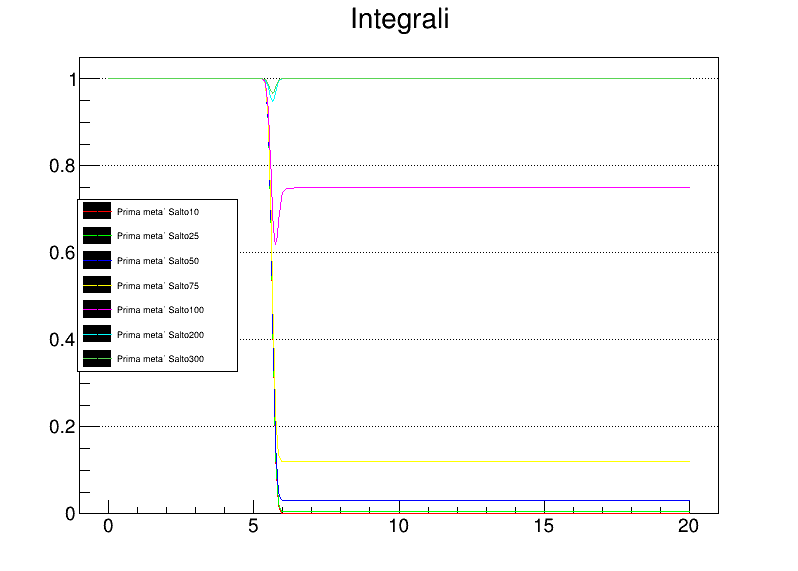
\includegraphics[width=0.7\linewidth]{IMG/SaltoR}
  \caption{I pesi dell'integrale della prima met\`a del dominio per $\sigma=0.5$}\label{fig:SaltoR}
\end{figure}

Come si pu\`o notare dalla \autoref{tab:SaltoDati} sebbene stia simulando un pacchetto d'onda in movimento e non un un'onda piana il peso dei coefficienti ricalca abbastanza bene i coefficienti teorici, e sembra avvicinarli di pi\`u man mano che allargo il pacchetto. Notare che la simulazione si allontana dalla teoria per le onde piane pi\`u si \`e vicini al regime in cui il potenziale \`e maggiore dell'energia dell'onda.

\begin{figure}[hbt]
  \centering
  \begin{tikzpicture}
    \begin{axis}[axis x line = center, axis y line = center, ylabel=R, ylabel style={left}, xlabel=E/V, xlabel style={below right}, xmin = -0.1, xmax = 10.1, ymin=-0.1,ymax =1.1]
      \addplot table[x=ev,y=fhS1] {Dati/pesi2.tdt};%{Dati/Salto.tdt};
      \addlegendentry{$\sigma=0.5$}
      \addplot table[x=ev,y=fhS2] {Dati/pesi2.tdt};
      \addlegendentry{$\sigma=1$}
      \addplot table[x=ev,y=fhS3] {Dati/pesi2.tdt};
      \addlegendentry{$\sigma=2$}
      \addplot table[x=ev,y=fhS4] {Dati/pesi2.tdt};
      \addlegendentry{$\sigma=4$}
      \addplot[domain=0:10, samples =501, green]	plot[id=Refl2]	function{x<1?1:1-(4*sqrt(x-1)*sqrt(x))/((sqrt(-1+x)+sqrt(x))*(sqrt(-1+x)+sqrt(x)))};
      \addlegendentry{teoria}
    \end{axis}
  \end{tikzpicture}
  \caption{La visualizzazione dei dati e il confronto con la teoria}
\end{figure}

\subsection{La barriera rettangolare}
Similmente a prima usiamo le definizioni dei $k$ in \eqref{eq:Ks}. Il potenziale avr\`a la forma:

\begin{equation}
  \lr\{.{\begin{array}{lr}
      V_0& 0<x<a\\
      0&\text{altrove}
  \end{array}}
\end{equation}
Per l'esempio $x_0=0$.

Dato che il potenziale ha una discontinuit\`a finita in $0$ e in $a$, funzione e derivata devono essere continue. Come prima:
\begin{equation}
  \lr\{.{\begin{array}{lr}
      A_\to e^{ik_1x} + A_\from e^{-ik_1x}	&	x<0\\
      C_\to e^{ik_2x} + C_\from e^{-ik_2x}	&	0<x<a\\
      B_\to e^{ik_1x} + B_\from e^{-ik_1x}	&	x>a
  \end{array}}\Rightarrow\lr\{.{\begin{array}{lr}
      A_\to  +A_\from = C_\to+C_\from															&	\text{in }0\\
      C_\to e^{ik_2a}+C_\from e^{-ik_2a} = B_\to e^{ik_1a} +B_\from e^{-ik_1a}				&	\text{in }a\\
      k_1\lrt{A_\to e^{-ik_1a}-A_\from e^{ik_1a}}=k_2\lrt{C_\to e^{-ik_2a}-C_\from e^{ik_2a}}	&	\text{in }0\\
      k_2\lrt{C_\to e^{ik_2a}-C_\from e^{-ik_2a}}=k_1\lrt{B_\to e^{ik_1a}-B_\from e^{-ik_1a}}	&	\text{in }a
  \end{array}}
\end{equation}
nel caso pi\`u generico. Nel nostro caso invece consideriamo un'onda piana da $-\infty$ che si muove verso destra prima di incontrare la barriera:
\begin{equation}
  \lr\{.{\begin{array}{ccc}
      A_\to = 1&,&
      A_\from = r\\
      B_\to = t&,&
      B_\from=0\\
      C_\to = m_1&,&
      C_\from=m_2
  \end{array}} \Rightarrow\lr\{.{\begin{array}{l}
      1+r= m_1 +m_2 \\
      m_1 e^{ik_2a}+m_2 e^{-ik_2a} = t e^{ik_1a}\\
      k_1\lrt{1 - r}=k_2\lrt{m_1 - m_2}\\
      k_2\lrt{m_1 e^{ik_2a}-m_2 e^{-ik_2a}}=k_1 t e^{ik_1a}
  \end{array}} \Rightarrow\lr\{.{\begin{array}{l}
      r	= \frac{\lrt{e^{2 i a k_2}-1}\lrt{k_1^2-k_2^2}}{\lrt{k_1-k_2}^2 e^{2 i a k_2}-\lrt{k_1+k_2}^2}\\
      t	= \frac{4 e^{-i a \lrt{k_1-k_2}} k_1 k_2}{\lrt{k_1+k_2}^2-\lrt{k_1-k_2}^2 e^{2 i a k_2}}\\
      m_1	= \frac{2k_1\lrt{k_1+k_2}}{\lrt{k_1+k_2}^2-\lrt{k_1-k_2}^2 e^{2 i a k_2}}\\
      m_2	= \frac{2 e^{2 i a k_2}k_1\lrt{k_2-k_1}}{\lrt{k_1+k_2}^2-\lrt{k_1-k_2}^2 e^{2 i a k_2}}
  \end{array}}
\end{equation}

ma a noi interessano:

\begin{equation}
  \lr\{.{\begin{array}{l}
      R = \lr||{r}^2 = \lr||{\frac{\sin\lrt{a k_2}\lrt{k_1^2-k_2^2}}{\lrt{k_1+k_2}^2 \sin\lrt{a k_2}+2 i k_1 k_2 \cos\lrt{a k_2}}}^2=
      \frac{\lrt{k_1^2-k_2^2}^2\sin^2\lrt{a k_2}}{4 k_1^2 k_2^2 \cos^2\lrt{a k_2}+\lrt{k_1^2+k_2^2}^2\sin^2\lrt{a k_2}}\\
      T = \lr||{t}^2 = \lr||{\frac{2e^{-i a k_1}k_1 k_2}{i\lrt{k_1+k_2}^2 \sin\lrt{a k_2}-2k_1 k_2 \cos\lrt{a k_2}}}^2=
      \frac{4 k_1^2 k_2^2}{4 k_1^2 k_2^2 \cos^2\lrt{a k_2}+\lrt{k_1^2+k_2^2}^2\sin^2\lrt{a k_2}}
  \end{array}}
\end{equation}

Che messi in termini di $E$ e $V$ ed $m$:
%k_1 = \sqrt{2m E}
%k_2 = \sqrt{2m \lrt{E-V_0}}
\begin{equation}
  \lr\{.{\begin{array}{l}
      R = \frac{V_0^2\sin^2\lrt{a \sqrt{2m \lrt{E-V_0}}}}
      {4 \lrt{E^2 - EV_0} +V_0^2\sin^2\lrt{a \sqrt{2m \sqrt{E-V_0}}}}\\
      T = \frac{4 E\lrt{E-V_0}}
      {4 \lrt{E^2 - EV_0} +V_0^2\sin^2\lrt{a \sqrt{2m \sqrt{E-V_0}}}}
  \end{array}}
\end{equation}

\begin{figure}[hbt]
  \centering
  \begin{tikzpicture}
    \def \a {2}
    \begin{axis}[axis x line = center, axis y line = center, ylabel=R, ylabel style={left}, xlabel=E/V, xlabel style={below right}, xmin = -0.1, xmax = 10.1, ymin=-0.1,ymax =1.1]
      \addplot table[x=ev,y=L2] {Dati/pesiMurog1.tdt};%{Dati/Salto.tdt};
      \addlegendentry{$a=2,~\sigma = 0.5$}
      %	\addplot table[x=ev,y=L4] {Dati/pesiMurog1.tdt};
      %	\addlegendentry{$4$}
      \addplot table[x=ev,y=L2] {Dati/pesiMurog2.tdt};
      \addlegendentry{$a=2,~\sigma = 1$}
      \addplot table[x=ev,y=L2] {Dati/pesiMurog3.tdt};
      \addlegendentry{$a=2,~\sigma = 2$}
      \addplot table[x=ev,y=L2] {Dati/pesiMurog4.tdt};
      \addlegendentry{$a=2,~\sigma = 4$}
      %	\addplot table[x=ev,y=L2] {Dati/pesiMurog2.tdt};
      %	\addlegendentry{$4$}
      %	\addplot table[x=ev,y=L16] {Dati/pesiM.tdt};
      %	\addlegendentry{$16$}
      %(2*sin(20*a*sqrt(5 - 5/x))*sin(20*a*sqrt(5 - 5/x)))/(1 - 8*x + 8*x*x - cos(40*a*sqrt(5 - 5/x)))
      \addplot[domain=1.00000001:10, samples =501, blue]	plot[id=MRefl2]	function{(2*sin(20*\a*sqrt(5 - 5/x))*sin(20*\a*sqrt(5 - 5/x)))/(1 - 8*x + 8*x*x - cos(40*\a*sqrt(5 - 5/x)))};
      \addlegendentry{teoria $a=2$ }
      %	\addplot[domain=1.00000001:10, samples =501, green]	plot[id=MRefl2]	function{(2*sin(20*4*sqrt(5 - 5/x))*sin(20*4*sqrt(5 - 5/x)))/(1 - 8*x + 8*x*x - cos(40*4*sqrt(5 - 5/x)))};
      %	\addlegendentry{teoria 4 }
      %	\addplot[domain=0:10, samples =501, red]	plot[id=MRefl2]	function{(-2*sin(4*sqrt(-1 + x))*sin(4*sqrt(-1 + x)))/(-1 + 8*x - 8*x*x + cos(2*4*sqrt(-1 + x)))};
      %	\addlegendentry{teoria 4}
      %	\addplot[domain=0:10, samples =501, green]	plot[id=MRefl2]	function{(-2*sin(8*sqrt(-1 + x))*sin(8*sqrt(-1 + x)))/(-1 + 8*x - 8*x*x + cos(2*8*sqrt(-1 + x)))};
      %	\addlegendentry{teoria 8}
    \end{axis}
  \end{tikzpicture}
  \caption{La visualizzazione dei dati e il confronto con la teoria}
\end{figure}

\begin{figure}[hbt]
  \centering
  \begin{subfigure}[b]{0.49\textwidth}
    \begin{tikzpicture}
      \def \a {2}
      \begin{axis}[axis x line = center, axis y line = center, ylabel=R, ylabel style={left}, xlabel=E/V, xlabel style={below right}, xmin = 1.9, xmax = 4.1, ymin=-0.001,ymax = 0.11]
	\addplot table[x=ev,y=S05] {Dati/DataOsc2.tdt};
	\addlegendentry{$a=2$, $\sigma=0.5$};
	\foreach \s in {1,2,3}{
	  \addplot table[x=ev,y=S\s] {Dati/DataOsc2.tdt};
	  \edef\temp{\noexpand\addlegendentry{$a=2$, $\sigma=\s$}}
	  \temp
	}
	\addplot[domain=2:4, samples =501, blue]	plot[id=MRefl2z]	function{(2*sin(20*\a*sqrt(5 - 5/x))*sin(20*\a*sqrt(5 - 5/x)))/(1 - 8*x + 8*x*x - cos(40*\a*sqrt(5 - 5/x)))};
	\addlegendentry{teoria a=\a}
	\addplot[domain=2:4, samples =501, red]	plot[id=Refl2]	function{x<1?1:(-1+sqrt(1-1/x))*(-1+sqrt(1-1/x))/((1+sqrt(1-1/x))*(1+sqrt(1-1/x)))};
	\addlegendentry{teoria scalino}
      \end{axis}
    \end{tikzpicture}
  \end{subfigure}
  ~~
  \begin{subfigure}[b]{0.49\textwidth}
    \begin{tikzpicture}
      \def \a {2}
      \begin{axis}[axis x line = center, axis y line = center, ylabel=R, ylabel style={left}, xlabel=E/V, xlabel style={below right}, xmin = 1.9, xmax = 4.1, ymin=-0.001,ymax = 0.11]
	\foreach \s in {4,5,6,7}{
	  \addplot table[x=ev,y=S\s] {Dati/DataOsc2.tdt};
	  \edef\temp{\noexpand\addlegendentry{$a=2$, $\sigma=\s$}}
	  \temp
	}
	\addplot[domain=2:4, samples =501, blue]	plot[id=MRefl2z]	function{(2*sin(20*\a*sqrt(5 - 5/x))*sin(20*\a*sqrt(5 - 5/x)))/(1 - 8*x + 8*x*x - cos(40*\a*sqrt(5 - 5/x)))};
	\addlegendentry{teoria a=\a}
      \end{axis}
    \end{tikzpicture}
  \end{subfigure}
  \caption{I dati tra 2 e 4 per una barriera larga 2}
\end{figure}


\begin{figure}[hbt]
  \centering
  \begin{subfigure}[b]{0.49\textwidth}
    \begin{tikzpicture}
      \def \a {4}
      \begin{axis}[axis x line = center, axis y line = center, ylabel=R, ylabel style={left}, xlabel=E/V, xlabel style={below right}, xmin = 1.9, xmax = 4.1, ymin=-0.001,ymax = 0.11]
	\addplot table[x=ev,y=S05] {Dati/DataOsc4.tdt};
	\addlegendentry{$a=4$, $\sigma=0.5$};
	\foreach \s in {1,2,3}{
	  \addplot table[x=ev,y=S\s] {Dati/DataOsc4.tdt};
	  \edef\temp{\noexpand\addlegendentry{$a=4$, $\sigma=\s$}}
	  \temp
	}
	\addplot[domain=2:4, samples =501, blue]	plot[id=MRefl2z]	function{(2*sin(20*\a*sqrt(5 - 5/x))*sin(20*\a*sqrt(5 - 5/x)))/(1 - 8*x + 8*x*x - cos(40*\a*sqrt(5 - 5/x)))};
	\addlegendentry{teoria a=\a}
	\addplot[domain=2:4, samples =501, red]	plot[id=Refl2]	function{x<1?1:(-1+sqrt(1-1/x))*(-1+sqrt(1-1/x))/((1+sqrt(1-1/x))*(1+sqrt(1-1/x)))};
	\addlegendentry{teoria scalino}
      \end{axis}
    \end{tikzpicture}
  \end{subfigure}
  ~~
  \begin{subfigure}[b]{0.49\textwidth}
    \begin{tikzpicture}
      \def \a {4}
      \begin{axis}[axis x line = center, axis y line = center, ylabel=R, ylabel style={left}, xlabel=E/V, xlabel style={below right}, xmin = 1.9, xmax = 4.1, ymin=-0.001,ymax = 0.11]
	\foreach \s in {4,5,6,7}{
	  \addplot table[x=ev,y=S\s] {Dati/DataOsc4.tdt};
	  \edef\temp{\noexpand\addlegendentry{$a=4$, $\sigma=\s$}}
	  \temp
	}
	\addplot[domain=2:4, samples =501, blue]	plot[id=MRefl2z]	function{(2*sin(20*\a*sqrt(5 - 5/x))*sin(20*\a*sqrt(5 - 5/x)))/(1 - 8*x + 8*x*x - cos(40*\a*sqrt(5 - 5/x)))};
	\addlegendentry{teoria a=\a}
      \end{axis}
    \end{tikzpicture}
  \end{subfigure}
  \caption{I dati tra 2 e 4 per una barriera larga 4}
\end{figure}

\begin{figure}[hbt]
  \centering
  \begin{subfigure}[b]{0.49\textwidth}
    \begin{tikzpicture}
      \def \a {0.1};
      \def \m {5};
      
      \begin{axis}[axis x line = center, axis y line = center, ylabel=R, ylabel style={left}, xlabel=E/V, xlabel style={below right}, xmin = 0.25, xmax = 1.75, ymin=-0.1,ymax =1.1]
	\def \En {25};
	\addplot table[x=ev,y=E25] {Dati/datatunnelm5.tdt};
	\addlegendentry{S: $E=25$}
	\addplot[domain=0.25:1.75, samples =501, orange]	plot[id=MTunnel525]	function{(x==1)?1-2/(2+\a*\a*\En*\m):1+(8*(x-1)*x)/(cos(2*\a*sqrt(2*\m*\En*(x-1)))-1-8*x*(x-1))};
	\addlegendentry{T: $E=25$}
	\def \En {75};
	\addplot table[x=ev,y=E75] {Dati/datatunnelm5.tdt};
	\addlegendentry{S: $E=75$}
	\addplot[domain=0.25:1.75, samples =501, green]	plot[id=MTunnel575]	function{(x==1)?1-2/(2+\a*\a*\En*\m):1+(8*(x-1)*x)/(cos(2*\a*sqrt(2*\m*\En*(x-1)))-1-8*x*(x-1))};
	\addlegendentry{T: $E=75$}
      \end{axis}
    \end{tikzpicture}
  \end{subfigure}
  ~
  \begin{subfigure}[b]{0.49\textwidth}
    \begin{tikzpicture}
      \def \a {0.1};
      \def \m {5};
      
      \begin{axis}[axis x line = center, axis y line = center, ylabel=R, ylabel style={left}, xlabel=E/V, xlabel style={below right}, xmin = 0.25, xmax = 1.75, ymin=-0.1,ymax =1.1]
	\def \En {50};
	\addplot table[x=ev,y=E50] {Dati/datatunnelm5.tdt};
	\addlegendentry{S: $E=50$}
	\addplot[domain=0.25:1.75, samples =501, orange]	plot[id=MTunnel550]	function{(x==1)?1-2/(2+\a*\a*\En*\m):1+(8*(x-1)*x)/(cos(2*\a*sqrt(2*\m*\En*(x-1)))-1-8*x*(x-1))};
	\addlegendentry{T: $E=50$}
	\def \En {100};
	\addplot table[x=ev,y=E100] {Dati/datatunnelm5.tdt};
	\addlegendentry{S: $E=100$}
	\addplot[domain=0.25:1.75, samples =501, green]	plot[id=MTunnel5100]	function{(x==1)?1-2/(2+\a*\a*\En*\m):1+(8*(x-1)*x)/(cos(2*\a*sqrt(2*\m*\En*(x-1)))-1-8*x*(x-1))};
	\addlegendentry{T: $E=100$}
      \end{axis}
    \end{tikzpicture}
  \end{subfigure}
  \caption{Provo a simulare l'effetto tunnel, impiegando un pacchetto con $\sigma = 4$, con massa delle particelle 5 e spessore della barriera $a=0.1$}
\end{figure}

\begin{figure}[hbt]
  \centering
  \begin{subfigure}[b]{0.49\textwidth}
    \begin{tikzpicture}
      \def \a {0.1};
      \def \m {10};
      
      \begin{axis}[axis x line = center, axis y line = center, ylabel=R, ylabel style={left}, xlabel=E/V, xlabel style={below right}, xmin = 0.25, xmax = 1.75, ymin=-0.1,ymax =1.1]
	\def \En {25};
	\addplot table[x=ev,y=E25] {Dati/datatunnelm10.tdt};
	\addlegendentry{S: $E=25$}
	\addplot[domain=0.25:1.75, samples =501, orange]	plot[id=MTunnel525]	function{(x==1)?1-2/(2+\a*\a*\En*\m):1+(8*(x-1)*x)/(cos(2*\a*sqrt(2*\m*\En*(x-1)))-1-8*x*(x-1))};
	\addlegendentry{T: $E=25$}
	\def \En {75};
	\addplot table[x=ev,y=E75] {Dati/datatunnelm10.tdt};
	\addlegendentry{S: $E=75$}
	\addplot[domain=0.25:1.75, samples =501, green]	plot[id=MTunnel575]	function{(x==1)?1-2/(2+\a*\a*\En*\m):1+(8*(x-1)*x)/(cos(2*\a*sqrt(2*\m*\En*(x-1)))-1-8*x*(x-1))};
	\addlegendentry{T: $E=75$}
      \end{axis}
    \end{tikzpicture}
  \end{subfigure}
  ~
  \begin{subfigure}[b]{0.49\textwidth}
    \begin{tikzpicture}
      \def \a {0.1};
      \def \m {10};
      
      \begin{axis}[axis x line = center, axis y line = center, ylabel=R, ylabel style={left}, xlabel=E/V, xlabel style={below right}, xmin = 0.25, xmax = 1.75, ymin=-0.1,ymax =1.1]
	\def \En {50};
	\addplot table[x=ev,y=E50] {Dati/datatunnelm10.tdt};
	\addlegendentry{S: $E=50$}
	\addplot[domain=0.25:1.75, samples =501, orange]	plot[id=MTunnel550]	function{(x==1)?1-2/(2+\a*\a*\En*\m):1+(8*(x-1)*x)/(cos(2*\a*sqrt(2*\m*\En*(x-1)))-1-8*x*(x-1))};
	\addlegendentry{T: $E=50$}
	\def \En {100};
	\addplot table[x=ev,y=E100] {Dati/datatunnelm10.tdt};
	\addlegendentry{S: $E=100$}
	\addplot[domain=0.25:1.75, samples =501, green]	plot[id=MTunnel5100]	function{(x==1)?1-2/(2+\a*\a*\En*\m):1+(8*(x-1)*x)/(cos(2*\a*sqrt(2*\m*\En*(x-1)))-1-8*x*(x-1))};
	\addlegendentry{T: $E=100$}
      \end{axis}
    \end{tikzpicture}
  \end{subfigure}
  \caption{Provo a simulare l'effetto tunnel, impiegando un pacchetto con $\sigma = 4$, con massa delle particelle 10 e spessore della barriera $a=0.1$}
\end{figure}

Dai dati sembra che pi\`u la barriera \`e  grande rispetto alla larghezza del treno pi\`u la simulazione si allontana dalla teoria per le onde piane. Probabilmente questo \`e dovuto al fatto che con una barriera pi\`u grande del pacchetto questo si comporti con essa come se fosse in presenza di un salto di potenziale.

\begin{figure}[hbt]
  \centering
  \begin{subfigure}[b]{0.49\textwidth}
    \begin{tikzpicture}
      \def \a {0.1};
      \def \m {15};
      
      \begin{axis}[axis x line = center, axis y line = center, ylabel=R, ylabel style={left}, xlabel=E/V, xlabel style={below right}, xmin = 0.25, xmax = 1.75, ymin=-0.1,ymax =1.1]
	\def \En {25};
	\addplot table[x=ev,y=E25] {Dati/datatunnelm15.tdt};
	\addlegendentry{S: $E=25$}
	\addplot[domain=0.25:1.75, samples =501, orange]	plot[id=MTunnel525]	function{(x==1)?1-2/(2+\a*\a*\En*\m):1+(8*(x-1)*x)/(cos(2*\a*sqrt(2*\m*\En*(x-1)))-1-8*x*(x-1))};
	\addlegendentry{T: $E=25$}
	\addplot table[x=ev,y=E75] {Dati/datatunnelm15.tdt};
	\addlegendentry{S: $E=75$}
	\def \En {75};
	\addplot[domain=0.25:1.75, samples =501, green]	plot[id=MTunnel575]	function{(x==1)?1-2/(2+\a*\a*\En*\m):1+(8*(x-1)*x)/(cos(2*\a*sqrt(2*\m*\En*(x-1)))-1-8*x*(x-1))};
	\addlegendentry{T: $E=75$}
      \end{axis}
    \end{tikzpicture}
  \end{subfigure}
  ~
  \begin{subfigure}[b]{0.49\textwidth}
    \begin{tikzpicture}
      \def \a {0.1};
      \def \m {15};
      
      \begin{axis}[axis x line = center, axis y line = center, ylabel=R, ylabel style={left}, xlabel=E/V, xlabel style={below right}, xmin = 0.25, xmax = 1.75, ymin=-0.1,ymax =1.1]
	\def \En {50};
	\addplot table[x=ev,y=E50] {Dati/datatunnelm15.tdt};
	\addlegendentry{S: $E=50$}
	\addplot[domain=0.25:1.75, samples =501, orange]	plot[id=MTunnel550]	function{(x==1)?1-2/(2+\a*\a*\En*\m):1+(8*(x-1)*x)/(cos(2*\a*sqrt(2*\m*\En*(x-1)))-1-8*x*(x-1))};
	\addlegendentry{T: $E=50$}
	\def \En {100};
	\addplot table[x=ev,y=E100] {Dati/datatunnelm15.tdt};
	\addlegendentry{S: $E=100$}
	\addplot[domain=0.25:1.75, samples =501, green]	plot[id=MTunnel5100]	function{(x==1)?1-2/(2+\a*\a*\En*\m):1+(8*(x-1)*x)/(cos(2*\a*sqrt(2*\m*\En*(x-1)))-1-8*x*(x-1))};
	\addlegendentry{T: $E=100$}
      \end{axis}
    \end{tikzpicture}
  \end{subfigure}
  \caption{Provo a simulare l'effetto tunnel, impiegando un pacchetto con $\sigma = 4$, con massa delle particelle 15 e spessore della barriera $a=0.1$}
\end{figure}